\begin{figure}[htbp]
    \centering
    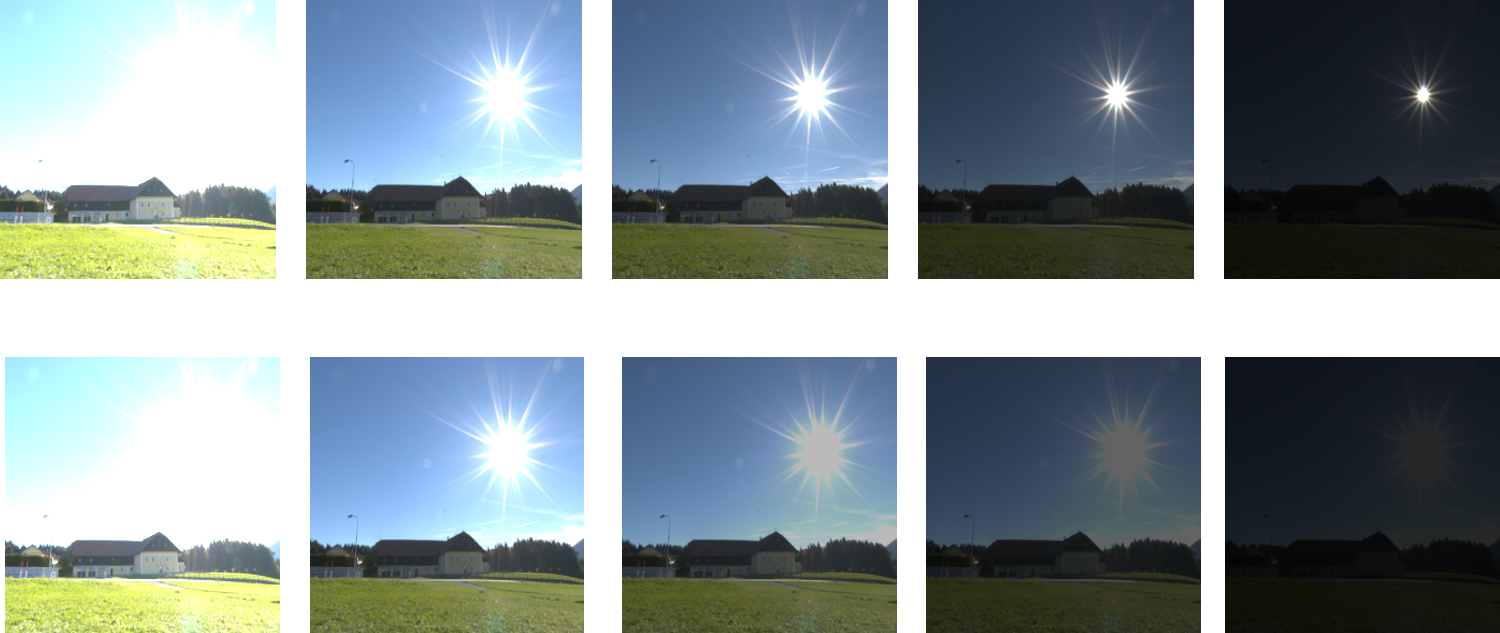
\includegraphics[width=1.0\textwidth]{Img/exposure-change.png}
    \caption[LDR图片与HDR图片在调整曝光时的不同]
    {调整LDR和HDR图像曝光的结果。第一行是从一幅HDR开始,不断减小场景曝光值;第二行则是对LDR执行同样的操作。可以看出对于HDR图像,多次降低曝光后太阳位置的亮度依然很亮,这说明HDR图像中太阳对应的像素值远远高于周边像素,与真实场景的光照情况一致。而LDR图像在降低曝光后,太阳位置的像素值会和周围像素一起降低,这显然是不符合真实光照条件的。}
    \label{fig:exposure-change}
\end{figure}